\documentclass[11pt]{article}
%\usepackage[firstpage]{draftwatermark}
\usepackage{times}
\usepackage{pdfpages}
\usepackage{fullpage}
\usepackage{url}
\usepackage{hyperref}
\usepackage{fancyhdr}
\usepackage{graphicx}
\usepackage{tabularx}
\usepackage{enumitem}
\usepackage{indentfirst}
\usepackage{subcaption}
\usepackage{amsmath, amssymb}
\DeclareMathOperator*{\argmax}{arg\,max}
\DeclareMathOperator*{\argmin}{arg\,min}
\usepackage{units}
\usepackage{IEEEtrantools}

% Added by crv
\usepackage{algorithm}
\usepackage{algorithmic}
\usepackage{siunitx}
\usepackage{multirow}
% \usepackage{minitab}
\newcommand{\minitab}[2][l]{\begin{tabular}{#1}#2\end{tabular}}

% Added by bsb
\usepackage{color,soul}
\DeclareRobustCommand{\hlr}[1]{{\sethlcolor{red}\hl{#1}}}
\DeclareRobustCommand{\hlg}[1]{{\sethlcolor{green}\hl{#1}}}
\DeclareRobustCommand{\hlb}[1]{{\sethlcolor{blue}\hl{#1}}}
\DeclareRobustCommand{\hly}[1]{{\sethlcolor{yellow}\hl{#1}}}

\setcounter{secnumdepth}{4}
\graphicspath{{images/}}
\pagestyle{fancy}

\newcommand{\doctitle}{Modeling single-beam sonar with Gazebo ray tracing}

\addtolength{\headheight}{2em}
\addtolength{\headsep}{1.5em}
\lhead{\doctitle}
\rhead{}

\newcommand{\capt}[1]{\caption{\small \em #1}}

\cfoot{\small Brian Bingham \today \\ \thepage}
\renewcommand{\footrulewidth}{0.4pt}

\newenvironment{xitemize}{\begin{itemize}\addtolength{\itemsep}{-0.75em}}{\end{itemize}}
\newenvironment{tasklist}{\begin{enumerate}[label=\textbf{\thesubsubsection-\arabic*},ref=\thesubsubsection-\arabic*,leftmargin=*]}{\end{enumerate}}
\newcommand\todo[1]{{\bf TODO: #1}}
\setcounter{tocdepth}{2}
\setcounter{secnumdepth}{4}

\makeatletter
\newcommand*{\compress}{\@minipagetrue}
\makeatother

%\renewcommand{\chaptername}{Volume}
%\renewcommand{\thesection}{\Roman{section}}
%\renewcommand{\thesubsection}{\Roman{section}-\Alph{subsection}}

\begin{document}

% More verticle spacing in eqnarray
\setlength{\IEEEnormaljot}{10pt}%


% set the figure default size
\newcommand{\SF}{0.7}
\newcommand{\SFb}{0.45}
\newcommand{\SFPic}{0.45}
\newcommand{\SFPlot}{0.45}
\newcommand{\SFc}{0.52}
% Just a lazy way of setting the figure width (percentage of text width)
% 0.7 works well for 1 column
% 0.4 works well for 2 column
\newcommand{\FigWidth}{\SF}


\newpage
% Title Page
\setcounter{page}{1}
\begin{center}
{\huge \doctitle}\footnote{Document source at \url{https://www.overleaf.com/read/tcxjgnmqphwj} and \url{https://github.com/bsb808/OceanNotes}}
\end{center}

%\begin{abstract}
%Abstract
%\end{abstract}
\section{Introduction}
The complexity of the sea poses difficulties in effective communication and navigation which makes it difficult to achieve full autonomy in UUVs. 

The risk that unreliable communications or navigation posed by unmanned vehicles continues to be an issue.

In-situ or field testing is required to validate a new technology, control algorithm, or proof-of-concept. 

Difficult environments and other factors can sometimes cause delays in testing, creating long periods of time between design and testing.

Simulation environments are useful tools for testing autonomous vehicles. 

They provide a cost-effective capability to provide rapid feedback on system updates, proof-of-concepts, etc.

Simulation is not a substitute for field testing.

Capturing the physics of the underwater environment is computationally expensive.

There are few simulators capable of simulating an underwater environment and fewer underwater sensors.

The motivation for this paper si to provide the underwater development community a sonar sensor model that can be used in research and development efforts for UUVs. 

We present a computationally efficient sonar sensor model and implementation that generates data consistent with experimental measurements typical of high-frequency forward-looking (FLS) and multibeam sonar (MBS) sensors.

The sonar sensor model includes several acoustic properties to capture underwater physical phenomena such as target strength (TS), transmission loss (TL), speckle noise, and scattering. These properties are captured in a point-scattering method developed in \cite{brown17point}.

Both point-scattering and beamforming are taken into account, making our implementation unique among sonar sensor models.

\section{Related Work}
Work has been published describing the development of a sonar simulation model.

Two of these have developed their models into supporting robotics framework.

In \cite{demarco15computationally} a Gazebo sonar sensor model is developed using ray tracing. The Gazebo ray-tracing functionality generates a 3D point cloud which is transformed into a sonar image. On inspection, the acoustic properties were either hard-coded or commented out and did not include speckle noise simulation.

In \cite{cerqueira17novel}, a GPU-based sonar simulator is developed using rasterization. They model two types of sonar: mechanically scanned imaging sonar (MSIS) and FLS. The acoustics features provided in their model are accurate and representative of sound propagation. The sonar sensor model is modeled using a virtual camera and utilizes the following three parameters to render the camera as sonar: pulse distance, echo intensity, and field-of-view. Physical tests were also conducted to compare the simulation results with the physical imaging sonar.

\begin{table}[]
    \centering
    \begin{tabular}{|c|c|c|c|}
         \hline
         Model & DeMarco et al. (2015) & Cerquiera et al. (2017) & Ours \\
         \hline
        \multirow{ 2}{*}{Sonar Type} & \multirow{ 2}{*}{FLS} & FLS & FLS  \\
        & & MSIS & MB\\ 
        \hline
        Rendering & Rasterization & Rasterization & Rasterization \\ 
        \hline
        % \multirow{5}{*}{Features} & & Reflection & Reflection \\
        % & & Speckle & Speckle \\
        % & Reflection & Attenuation & Attenuation \\
        % & Speckle & Surface Irregularities & Scattering \\
        % & & Reverberation & Beamforming \\
        \multirow{5}{*}{Features} & \multirow{5}{*}{\minitab[c]{Reflection \\ Speckle}} & Reflection & Reflection \\
        & & Speckle & Speckle \\
        & & Attenuation & Attenuation \\
        & & Surface Irregularities & Scattering \\
        & & Reverberation & Beamforming \\
        \hline
        \multirow{2}{*}{Evaluation} & Qualitative & Qualitative & Qualitative \\
        & Computation Time & Quantitative & Compuation Time \\
        \hline
    \end{tabular}
    \caption{Summary of Sonar Sensor Models}
    \label{tab:sonar_models}
\end{table}

\section{Approach}
The model is based on a ray-based spatial descretization of the model facets, beampattern appropriate for a line array, and a point scattering model of the echo level.

\subsection{Active Sonar Equation}
% When modeling a single sonar beam, only the far field is considered in an effort to maintain computational efficiency. The far field begins at a distance of $2\lambda$
With respect to a target of interest, the simplest form of the sonar equation is given as 
\begin{equation}
EL = SL - 2(TL)+ TS % = 10 \log\left( \frac{I_R}{I_T} \right)
\end{equation}
where echo level, $EL$, is the intensity of the returned signal which is a function of the source level, $SL$, two-way transmission loss, $TL$, and target strength, $TS$.

$SL$ is the sound pressure level at a distance of 1m from a sonar and is defined as the decibel of the ratio of the signal intensity, $I_0$, and a reference intensity, $I_{ref}$. A common $I_{ref}$ in underwater acoustics is a reference pressure of \SI{1}{\micro\pascal}. $SL$ is defined as
\begin{equation}
SL=10\log\frac{I_0}{I_{ref}}
\end{equation}

$TL$ is the attenuation of sound as it propagates a distance \SI{1}{\meter} from a sonar source to a range, $r$, from a source.
\begin{equation}
    TL=20\log\frac{r}{r_0}
\end{equation}
where $r_0$ is a reference range typically given as \SI{1}{\meter}. Attenuation loss can be due to absorption, scattering, and leakage from sound channels \cite{urick13principles}. Absorption loss can be modeled by the absorption coefficient, $a_c$, as
\begin{equation}
    a_c=\frac{A_1 P_1 f_1 f^2}{f_1^2 + f^2} + \frac{A_2 P_2 f_2 f^2}{f_1^2 + f^2} + A_3 P_3 f^2
\end{equation}
where $f$ is the transmitted frequency, $f_1$ and $f_2$ are the boric acid and magnesium sulfate relaxation frequencies, $A_1$, $A_2$, and $A_3$ are weighting amplitudes, $P_1$, $P_2$, and $P_3$ are nondimensional pressure correction factors \cite{francois82sound}. The attenuation coefficient is calculated by 
\begin{equation}
    \alpha_p = \frac{a_c \log 10}{20}
\end{equation}

The wave vector $k_w$ can be related to the attenuation via the overall attenuation which is modeled using a complex frequency-dependent relationship between the wave vector and the attenuation coefficient
\begin{equation}
    \label{eq:K}
    K = k_w + i\alpha_p
\end{equation}
where $k_w$ is defined as 
\begin{equation}
    k_w = \frac{2 \pi f}{c}
\end{equation}

According to \cite{urick13principles}, the combination of spherical spreading and absorption provides a reasonable approximation under a wide variety of conditions,
\begin{equation}
    TL=20 \log(r) + a_c r
\end{equation}

Target strength is defined as the ratio of intensity reflected, $I_r$ by an object at a distance of \SI{1}{\meter} from the object to the incident intensity, $I_i$,
\begin{equation}
    TS=10 \log\frac{I_r}{I_i}
\end{equation}
True target strength in water depends on a variety of parameters such as specular reflection, object aspect, surface irregularities, acoustic impedance, and internal structure and composition.

% \section{Beam Pattern Model}
% The background of modeling the beam pattern is covered by the following:
% \begin{itemize}
% \item \href{http://www.personal.psu.edu/faculty/m/x/mxm14/}{Martin Mazur's} 2012 Underwater Acoustics (Penn State) \href{http://www.personal.psu.edu/faculty/m/x/mxm14/sonar/Mazur-sonar_signal_processing_combined.pdf}{course notes}.
% \item John Leonard's \href{https://ocw.mit.edu/courses/mechanical-engineering/2-011-introduction-to-ocean-science-and-engineering-spring-2006/readings/hw5_sonar_leonar.pdf}{Introduction to Sonar} from Alex Techet's 2006 Introduction to Ocean Science and Engineering \href{https://ocw.mit.edu/courses/mechanical-engineering/2-011-introduction-to-ocean-science-and-engineering-spring-2006/}{course notes}.
% \item \href{https://www3.mbari.org/data/mbsystem/sonarfunction/SeaBeamMultibeamTheoryOperation.pdf}{SeaBeam Multibeam Sonar Theory of Operation}.
% \end{itemize}
\subsection{Single Beam Sonar Model}
A single sonar beam is modeled using discrete rays. The individual rays are indexed as $i=\{1, 2, ... N\}$ for $N$ rays. The following information is generated for each ray within an individual beam:
\begin{itemize}
    \item The range $r_i$ as the distance from the origin of the sonar reference frame to the first intersection between the ray and a target in the field of view. The azimuth of the ray is fixed in the sensor frame as $\theta_i$ and the inclination angle of the ray is $\phi_i$
    \item The incident angle $a_i$ as the difference between the ray vector, $\bold{z}$, and the normal vector, $\bold{n}$ of the target surface at the location of intersection between the ray vector and the target surface.
    \item The reflectivity of the target intersected by the $i^{th}$ ray, $\mu_i cos(\theta)$, which is a property of the target object model
\end{itemize}

\subsubsection{Ray-based Beam Model}
We define a ray as a vector, $\bold{z}$, from the sensor frame origin to the first intersection with a visual object within the scene. We calculate the incident angle, $\alpha_i$, as
% \begin{equation}
%     \psi_i = cos^{-1}\left( \frac{\bold{z_i} \cdot \bold{n_i}}{\|\bold{z_i}\|\|\bold{n_i}\|} \right)
% \end{equation}
% \begin{equation}
%     \psi_i = cos^{-1}(\bold{\hat{z}_i} \cdot \bold{\hat{n}_i})
% \end{equation}
\begin{equation}
    \alpha_i = 180^{\circ} - cos^{-1}(\bold{\hat{z}_i} \cdot \bold{\hat{n}_i})
\end{equation}
where $\bold{\hat{z}_i}$ and $\bold{\hat{n}_i}$ are the ray and normal direction unit vectors respectively.

The projected ray surface area, $dA$, is the area projected onto the visual object by the individual ray. If the changes in both $d\theta_i$ and $d\phi_i$ angles for each ray are assumed to be infinitesimally small, then the projected area ray scene can be calculated by
\begin{equation}
    dA = r_i^2 d \theta_i d \phi_i
\end{equation}
% However, $dS$ is the true surface area patch of the visual object. The following two relationships are used to calculate $dS$ for a more accurate surface area approximation:
% Need a better way to phrase this
The ray area projected onto a surface, $dS_i$ is a function of the incident angle, calculated as 
\begin{equation}
    dS_i = \frac{dA}{cos(\alpha_i)}
\end{equation}
and expressed as
\begin{equation}
    dS_i = \frac{r_i^2 d \theta_i d \phi_i}{cos(\alpha_i)}
\end{equation}

The target strength is given by 
\begin{equation}
    TS_i = 10 \log\frac{I_{ri}}{I_{Ii}}
\end{equation}
and using Lambert's reflection law, the ratio of intensities is
\begin{equation}
    \frac{I_{ri}}{I_{Ii}} = \mu cos^2(\alpha_i)dS_i
\end{equation}
% Not sure what \mu is representing here
Substituting for $dS_i$, the intensity ratio becomes
% Made changes to the following equation (cos^2 -> cos)
\begin{equation}
    \frac{I_{ri}}{I_{Ii}}= \mu cos(\alpha_i)r_i^2d\theta_id\phi_i
\end{equation}

The physical model defined by Equation \ref{eq:K} is simulated using a point-based scattering model developed in \cite{brown17point}. The model generates a spatially coherent time series that is useful in simulating narrowband sonar applications such as the FLS and MBS systems. The model uses discrete scatterers distributed over a surface. These scatterers are representative of the number of surfaces a ray intersects based on the object's surface mesh. In our model, this approach is computationally inefficient. Therefore, we define each ray in a beam as a scatterer. The overall spectrum of the signal received from each ray, $P(f)$, is computed as
\begin{equation}
    P(f)_i = \frac{S(f)\sum^N_{i=1}a_ie^{iKr_i}}{r_i^2}
\end{equation}
where $S(f)$ is the transmitted spectrum of the source, $N$ is the number of scatters, $a_i$ is the complex scatterer amplitude, and $f$ is a frequency vector. $P(F)$ is a combination of the physical model for echo level and a complex random scale factor for speckle noise resolved in the frequency domain.

The source level is a user defined input and remains constant for each ray and is modeled in the frequency domain by $S(f)$,
\begin{equation}
    S(f)_i = S_0e^{-(f-f_c)^2b^2\pi^2}
\end{equation}
% The source level is defined by $S_0$ and has units of \SI{}{\pascal\meter}. 
The frequency vector, $f$, is a linearly spaced vector from $f_{min}$ to $f_{max}$ and centered on the central frequency, $f_c$. The full width of the transmit spectrum is the bandwidth, $b$, a user provided input based on the sonar specifications. As an example, the bandwidth for the BlueView P900-45 FLS is \SI{2.95}{\kHz}
\begin{equation}
    f=f_{min} ... f_{max}
\end{equation}
\begin{equation}
    f_{min} = f_c - \frac{b}{2}
\end{equation}
\begin{equation}
    f_{max} = f_c + \frac{b}{2}
\end{equation}

Spherical spreading is an appropriate assumption for modeling transmission loss. The two-way transmission loss for incoherent scattering in $P(f)$ is captured in the denominator, $r_i^2$

The scatter amplitude, $a_i$, is calculated for each ray,
\begin{equation}
    a_i = \frac{\xi_{xi} + i \xi_{yi}}{\sqrt{2}}\sqrt{\mu cos^2(\alpha_i)r_i^2d\theta_id\phi_i}
\end{equation}
Although the random variable, $\xi_i$, is indexed by $i$ to represent the ray index, the real random variable and the complex random variable must both be generated and different from each other, hence the $x$ and $y$ notation. Overall, the random variables are representative of Gaussian noise and for our purposes, satisfies the speckle noise requirement \cite{brown17point}. The variables under the square root represent the target strength of an incident ray on an object.

% The discrete inverse Fourier transform of $P(f)$ transfers the function from the frequency domain to the time domain and results in a time series of the received signal \cite{oppenheim99discrete}.
% \begin{equation}
%     P(t_n)=\sum^N_{m=1}e^{-i2\pi f_mt_nP(f_m)\Delta f}
% \end{equation}

\subsection{Beam Pattern Geometry}
% The geometry of the beam pattern is illustrated in Figure~\ref{f:bpattern}.  Most of the energy in the beam pattern is in the \emph{main lobe} and the center of that lobe is the \emph{main response axis} (MRA), shown as the Main axis in the figure. The angle from the MRA to the \emph{half power point} is $\theta_w$ and the \emph{beam width} (Full angle in the Figure) is twice this value:
We combine the ray-based discretization of the single beam with a linear array beam pattern model. The beam pattern of an array is defined in polar coordinates where the acoustic intensity is the distance along the radial axis and the angle is relative to the transducer axis. The beam pattern is visualized as one main lobe in the center with smaller side lobes radiating away from the main axis. By inspection, the highest return will be along the main axis as the response decreases off-axis. Therefore, the echo level depends on the size and position of a target within a beam. The beam width, $\theta_{bw}$, is marked at \SI{-3}{\decibel} on the main lobe. We define half the beam width as 
\begin{equation}
    \theta_w = \frac{\theta_{bw}}{2}
\end{equation}
The beam pattern, $B(\theta)$, expresses the $EL$ as a function of $\theta$, the angle relative to the main axis
\begin{equation}
    EL = EL|B(\theta)|^2
\end{equation}

For a continuous line array of length $L$, radiating energy at a wavelength $\lambda$, the beam pattern is that of a uniform aperture function. The radiated power is modeled as a normalized $sinc$ function
\begin{equation}
    |B(Lu)|^2 = |sinc(Lu)|^2 = \begin{cases}
      1, & \mathrm{for}\: Lu = 0 \\
      \left| \frac{sin(\pi L u)}{\pi L u}\right|^2, & \mathrm{otherwise}
    \end{cases}
\end{equation}

where $u$ is the electrical angle
\begin{equation}
    u = \frac{sin(\theta)}{\lambda}
\end{equation}
The half intensity point, $\theta_w$, can be solved for by setting
\begin{equation}
    |B(\theta_w)|^2 = \left|\frac{sin\big(\pi\frac{L}{\lambda}sin(\theta_w)\big)}{\pi\frac{L}{\lambda}sin(\theta_w)}\right|^2 = \frac{1}{2}    
\end{equation}
For high frequency sonar, we can assume $L \gg \lambda$, and $\theta_w$ becomes 
\begin{equation}
    \frac{L}{\lambda} = \frac{0.884}{\theta_{bw}} = \frac{0.442}{\theta_w}
\end{equation}
The final beam pattern is 
\begin{equation}
    |B(\theta_w)|^2 = \left|\frac{sin\big(\pi\frac{0.884}{\theta_{bw}}sin(\theta)\big)}{\pi \frac{0.884}{\theta_{bw}}sin(\theta)}\right|^2
\end{equation}
% The resulting pattern is shown in Figure **11

The azimuth angle, $\theta$, is defined as rotation about the z sensor frame axis and the main axis is defined as coincident with the sensor frame z axis. The use of $N$ rays, with angular location distributed evenly between in the range $[-\theta_{min}, \theta_{max}]$ and the intensity is a function of $\theta$ for the main lobe only.

The radial dimension is descretized by considering $M$ samples within the interval $[R_{min}, R_{max}]$. The number of samples in the radial dimension is a function of the range interval and the range resolution $(dR)$ and can be expressed as 
\begin{equation}
    M=\left| \frac{R_{max} - R_{min}}{dR} \right|
\end{equation}

As an example, the BlueView P900-45 FLS has a specified range interval of 2-\SI{60}{\meter} with a range resolution of $dR=$ \SI{0.0254}{\meter} resulting in $M=$ 2283 samples per beam. 

% Single Beam Sampling Application
The single sonar beam model generates a single pair of range and intensity values, $(r,I)$, which is generated by taking a uniform sample of the beam pattern. Each sample is a ray at $\theta_k$ in the range $[-\theta_w, theta_w]$ with the associated range and intensity pair $(r_k, i_k)$. The set of ordered pairs from all rays is $R=\{(r_0,i_0),(r_1,i_1),...,(r_N,i_N)\}$.

Using a uniform weighted average to model the beam pattern effect, the echo level for the beam can be calculated as 
% Used overline here to match paper
\begin{equation}
    \overline{EL}=\overline{l}=\frac{\sum^N_{k=0}w_ki_k}{\sum^N_{k=0}w_k}
\end{equation}
The weights are determined from the beam pattern function and calculated as 
\begin{equation}
    w_k=|B(\theta_k)|^2
\end{equation}

%subsection MATLAB IMPLEMENTATION - not necessary for this doc unless as note
% Our implementation relies on the Gazebo/ROS framework. For the purposes of verification we use parameters consistent with the BlueView P900-45D
% Can whittle down usage of BlueView and make a statement early on stating that it will be used for all examples.
\begin{algorithm}
\caption{Sonar Model}
\begin{algorithmic}
\STATE $ray \leftarrow calculateRay(distance, \alpha)$
\STATE $S(f) \leftarrow calculateTransmitSpectrum(frequency)$
\FOR{$k=1:\mathrm{nBeams}$}
    \FOR{$i=1:\mathrm{nRays}$}
        \STATE $noise \leftarrow Gaussian(x,y)$
        \STATE $amplitude \leftarrow calculateAmplitude(noise, \alpha, distance)$
        \STATE $P(f) \leftarrow calculateReceiveSpectrum(S(f), amplitude, distance)$
    \ENDFOR
    \STATE $beampattern \leftarrow calculateBeamPattern(\theta)$
    \STATE $P(t) \leftarrow transformReceiveSpectrum$
    \STATE $P(t)modified \leftarrow calculateModifiedReceiveIntensity(P(t), beampattern)$
\ENDFOR
\STATE $SPL \leftarrow calculateSoundPressureLevel(P(t)modified)$
\end{algorithmic}
\end{algorithm}




% \begin{equation}
% \theta_{bw}=2 \theta_w
% \end{equation}

% \begin{figure}[hbt!]
%   \centering
%   \includegraphics[width=0.4\textwidth]{images/beampattern.png}
%   \caption{Beam pattern schematic from \url{http://www.acousticsunpacked.org/AcousticBackground/AcousticTransducers.html}}
%   \label{f:bpattern}
% \end{figure}
% The beam pattern expresses the echo level as a function $\theta$, the angle relative the the MRA, as
% \begin{equation}
% EL = \left| G(\theta) \right|^2
% \end{equation}

% \subsection{Line Array Beam Pattern}
% For a line array of length $L$, radiating energy at wavelenth $\lambda$, the beam pattern is that of the \emph{uniform aperature function}.  The radiated power is modeled as a \emph{normalized sinc function}
% \begin{equation}
% \left| G(L u) \right|^2 =  \left|\mathrm{sinc}(L u)\right|^2 = 
% \begin{cases}
%   1 & \text{for} \, \,  Lu = 0 \\
%  \left| \frac{\sin(\pi L u)}{\pi L u} \right|^2  & \text{otherwise}
%   \end{cases}
% \end{equation}
% where $u$ is the \emph{electrical angle}
% \begin{equation}
% u = \frac{\sin(\theta)}{\lambda}.
% \end{equation}
% We can solve for the half power point by setting
% \begin{equation}
% G(\theta_w) = \frac{\sin(\pi \frac{L}{\lambda} \sin(\theta_w))}{\pi \frac{L}{\lambda} \sin(\theta_w)} = \frac{1}{\sqrt{2}}.
% \end{equation}
% For conditions where $L >> \lambda$, which is typical of high-frequency sonar, the half power point is
% \begin{equation}
% \theta_{w} = 0.442 \frac{\lambda}{L} \,\, \unit[]{rad}.
% \end{equation}
% When given a beam width, $\theta_{bw} = 2 \theta_w$ we can solve for the length to wavelength ratio
% \begin{equation}
% \frac{L}{\lambda} = \frac{0.884}{\theta_{bw}} = \frac{0.442}{\theta_w}
% \end{equation}
% so that the beam pattern is
% \begin{equation}
% \left| G(\theta_w) \right|^2 = \left| \frac{\sin(\pi \frac{0.884}{\theta_{bw}} \sin(\theta))}{\pi \frac{0.884}{\theta_{bw}} \sin(\theta)} \right|^2
% \end{equation}
% where $\theta_{bw}$ is the beam width in radians.  Figures \ref{f:linebp_polar} and \ref{f:linebp}\footnote{Figure Python source code at \url{https://bitbucket.org/brian_bingham/ocean_notes/src/master/src/single_beam/beam_pattern.py}} illustrate this beam pattern for a range of $L/\lambda$ values.  The differences in the beam shape between $[-\theta_w,\theta_w]$ is sufficiently small to be neglected.

% \begin{figure}[hb!]
%   \centering
%   \begin{subfigure}[t]{0.5\textwidth}
%     \centering
%     \includegraphics[width=\textwidth]{src/single_beam/linebp_polar_ratio_c.png}
%     \caption{As ratio.}
%   \end{subfigure}%
%   ~ 
%   \begin{subfigure}[t]{0.5\textwidth}
%     \centering
%     \includegraphics[width=\textwidth]{src/single_beam/linebp_polar_db_c.png}
%     \caption{In dB.}
%   \end{subfigure}
%   \caption{Beam pattern in polar coordinates. }
%   \label{f:linebp_polar}
% \end{figure}


% \begin{figure}[hb!]
%   \centering
%   \begin{subfigure}[t]{0.5\textwidth}
%     \centering
%     \includegraphics[width=\textwidth]{src/single_beam/linebp_ratio.png}
%     \caption{As ratio.}
%   \end{subfigure}%
%   ~ 
%   \begin{subfigure}[t]{0.5\textwidth}
%     \centering
%     \includegraphics[width=\textwidth]{src/single_beam/linebp_db.png}
%     \caption{In dB.}
%   \end{subfigure}
%   \caption{Beam pattern in Cartesian coordinates. }
%   \label{f:linebp}
% \end{figure}

% \subsection{Sampling the Beam Pattern via Ray Tracking}

% For a single beam sonar the model generates a single range and intensity pair: $(\bar{r},\bar{i})$.  We generate this pair by a uniform sampling of the beam pattern as shown in Figure~\ref{f:bpsampled}.  Each sample is a ray at $\theta_k$ in the range $[-\theta_w, \theta_w]$ generating the range/intensity pair $(r_k,i_k)$.  The set of ordered pairs from all the rays is $R = \{(r_0,i_0),(r_1,r_1),\ldots,(r_N,i_n)\}$.

% \subsubsection{Beam Echo Level - Intensity}

% The intensity value for each ray is the echo level for that geometry, $i_k = EL_k$.  We use a weighted average to model the beam pattern effect
% \begin{equation}
% \bar{EL} = \bar{i} = \frac{ \sum_{k=0}^{N} w_k i_k }{\sum_{k=0}^N w_k}
% \end{equation}
% where the weights are determined from the beam pattern function
% \begin{equation}
% w_k = \left| G(\theta_k) \right|^2 = \left| \frac{\sin(\pi \frac{0.884}{\theta_{bw}} \sin(\theta_k))}{\pi \frac{0.884}{\theta_{bw}} \sin(\theta_k)} \right|^2
% \end{equation}

% \subsubsection{Beam Range}
% The single-beam range value is the ray length corresponding to the maximum intensity, i.e.,\footnote{Need to improve notation here.}
% \begin{equation}
% (\bar{r},i_{max}) = \max(R)
% \end{equation}


% \begin{figure}[hbt!]
%   \centering
%   \includegraphics[width=0.75\textwidth]{src/single_beam/single_beam_sampled_annote.png}
%   \caption{Beam pattern sampled}
%   \label{f:bpsampled}
% \end{figure}


% \subsection{Gazebo Beam Output}
% For each simulated beam, Gazebo should provide the set of ordered pairs of echo level and range for each ray used to sample the beam: $B= \{(r_0,EL_0),(r_1,EL_1),\ldots,(r_N,EL_n)\}$, where each echo level, $EL_k$, is the simulated echo level that takes into account
% \begin{itemize}
% \item The sonar equation model, including the effect of incidence angle on target strength and
% \item The beam pattern function as captured by the coefficient $w_k$.
% \end{itemize}



\setcounter{page}{1}
\bibliographystyle{IEEEtran}
\bibliography{ocean_notes}

\end{document}
\usepackage{hyperref}

